% ============================================================
% Compile by XeLaTeX
% Econ Pre Beamer - Template (RedU)
% Requires: RedU.sty in the same directory.
% ============================================================
\documentclass[fontset=none,aspectratio=169]{ctexbeamer}
\usepackage{ctex}
\usepackage{latexsym,amsmath,xcolor,multicol,booktabs,calligra}
\usepackage{amssymb,amsthm,amsbsy,amsfonts}
\usepackage{graphicx,listings,stackengine,float,verbatim,caption,subcaption,xeCJK}
\usepackage{fontspec}
\usepackage{hyperref}
\hypersetup{hypertex=true,linkcolor=themeaccent,urlcolor=themecite}
\usepackage{RedU}

\setmainfont{Times New Roman}
\setCJKmainfont[AutoFakeBold={2}]{KaiTi}
\newCJKfontfamily{\HeiTi}[AutoFakeBold={3.17}]{SimHei}
\newCJKfontfamily{\FangSong}[AutoFakeBold={3.17}]{STFangsong}
\newCJKfontfamily{\huawenxingkai}[AutoFakeBold={2.17}]{STXingkai}
\newCJKfontfamily{\yasong}[AutoFakeBold,AutoFakeSlant]{FZYaSong-DB-GBK}
\newCJKfontfamily{\yankai}[AutoFakeBold={2.17},AutoFakeSlant]{Slideqiuhong Regular}
\setCJKmonofont{FangSong}
\newfontfamily\chalkd{Times New Roman}[AutoFakeBold={2.17}]
\setbeamerfont{normal text}{family=\chalkd,series=\mdseries}
\setbeamerfont{alerted text}{family=\chalkd,series=\mdseries}
\setbeamerfont{frametitle}{family=\chalkd,series=\mdseries}
\AtBeginDocument{\usebeamerfont{normal text}}
\usefonttheme[onlymath]{serif}

\setbeamertemplate{blocks}[rounded][shadow=true]
\newcommand{\term}[1]{\textcolor{themeaccent}{\textbf{#1}}}
\newcommand{\scrpt}[1]{\textcolor{themecite}{\scriptsize #1}}

\author{Qian and Yao \\ (\textit{Working Paper}, 2025)}
\title{\textbf{Digital Transformation and Labor Productivity}}
\subtitle{}
\institute{汇报人：{ \yankai 方鸿渐}}
\date{\today}

\begin{document}
\begin{frame}\titlepage\end{frame}
\section{Overview}
\begin{frame}{Authors}
\begin{itemize}
\item \textbf{Zhongshu Qian} - Economist, Clayton University. \\ \scrpt{Macroeconomics and industrial organization.}
\item \textbf{Yao Lu} - Economist, Marsh Academy. \\ \scrpt{Development economics and digital economy.}
\end{itemize}
\end{frame}
\begin{frame}{Overview}
\begin{itemize}
\item \textbf{Research question}: What are the productivity gains from digital transformation for small-scale manufacturing?
\item \textbf{Context}: A randomized subsidy to cloud-based ERP adoption through local industrial parks in Jiangsu, China.
\item \textbf{Key finding}: Digitalization relaxes \term{coordination frictions} and raises model-implied welfare.
\end{itemize}
\end{frame}

% ---------- [plain] Figure ----------
\begin{frame}[plain]
\centering
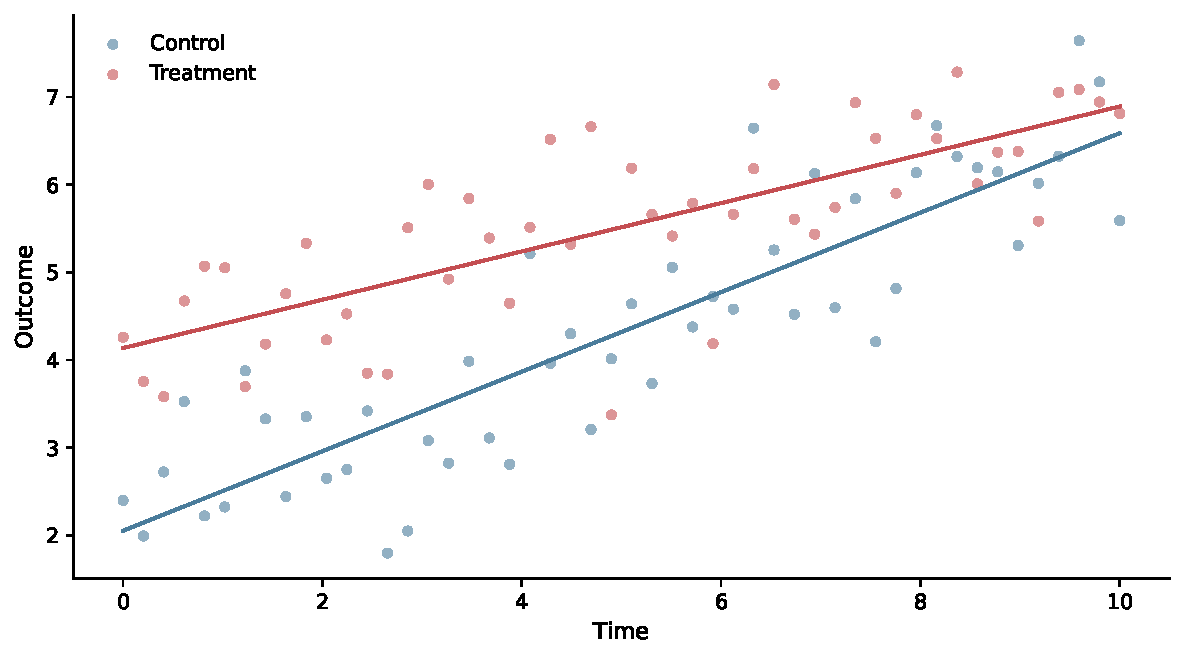
\includegraphics[width=0.88\paperwidth,height=0.86\paperheight,keepaspectratio]{fig/fig1.pdf}
\end{frame}

% ============================================================
% FIN
% ============================================================
\begin{frame}[plain]
    \begin{center}
\vspace{3em}
{\LARGE \color{themeaccent}\textbf{Thank You for Your Attention!}}

\vspace{3em}

{\color{halfgray}
{\yankai 方鸿渐}
\footnotesize
\quad 克莱登大学\ 哲学博士 \quad | \quad 
Clayton University\ PhD \\
微信：fanghongjian1898 \quad 邮箱：\texttt{fanghongjian1898@clayton.edu}
}
    \end{center}
\end{frame}

\end{document}
